% gopal nataraj thesis proposal
\documentclass[thesis]{../cls/thesis-umich}

% packages
\usepackage{subfiles} 	% partial compilation
\usepackage{

% title
\title{Statistical Methods for Quantitative MRI}

% author
\author{Gopal Nataraj}

% dept
\department{Electrical Engineering and Computer Science}

% year
\year=2016

% front piece
%\frontispiece{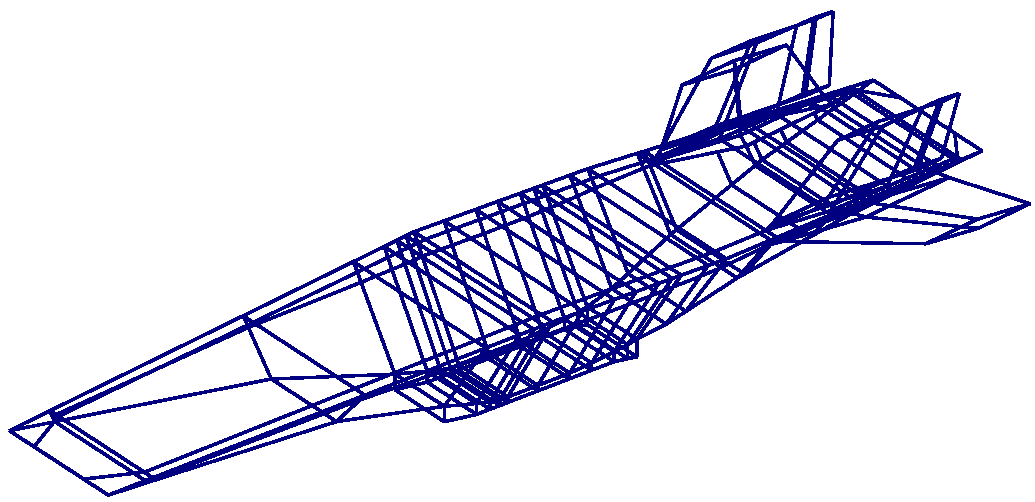
\includegraphics[width=4in]{./pics/frontispiece.pdf}}

% front page style
%\frontpagestyle{1}

% Dedication
%\dedication

% acknowledgments
% set width of acknowledgments as fraction of total \textwidth
%\acknowledgments[6]
%\acknowledgmentswidth{0.8}

% preface
%\preface[2]{ %
%}

% Committee
\committee{%
	Professor Jeffrey A. Fessler, Co-Chair \\
	Assistant Research Scientist Jon-Fredrik Nielsen, Co-Chair \\
	Professor Thomas Chenevert (?) \\
	Professor Alfred O. Hero III (?) \\
	Professor Douglas C. Noll (?) \\
	Associate Professor Clayton Scott (?)
}

% chair entered separately for formatting
\chair{%
	James F. Driscoll
}

% hide/show lists of figures, tables, etc.
\hidelistoftables
\hidelistofprograms
\hidelistofappendices

% Definition of any abbreviations used.
\abbreviations{
 \acro{CFD}{Computational Fluid Dynamics}
 \acro{MSRSF}{Monotonic, Single-Root Scalar Function}
}

% Some abstract text
\abstract{
We show that it is possible to get approximate solutions to
analytically intractable equations using iterative methods.  Thus we
show that the author could pass an undergraduate class in numerical
analysis.  In addition, a unique extension to Brent's method is
proposed that results in slight improvements in convergence.}
%\hideabstractpagenumber

%% DOCUMENT AREA
\begin{document}




\chapter{Introduction}   \label{chap:intro}
The first part.  For example in \ac{CFD}, which gives me a nice
example of an abbreviation to demonstrate, the equation of state
cannot be solved analytically when a perfect gas is not assumed.


\newpage

And this should at least continue onto a second page.  There are many
texts that have a section on the subject, for instance
\cite{chapra:2002:numerics}.

\chapter{Using This Template}   \label{chap:manual}
This chapter is stuck among the others as a brief users' manual for this
template.  The approach to this template is to result in \LaTeX~source
code files (\textit{i.e.}~\tfile{.tex} files) that are as simple as
possible.  It also tries to do as much as possible automatically so that
the user does not have to spend a lot of effort trying to match the
confusing and arbitrary guidelines from Rackham.  This is particularly
useful for the first few pages, for example the title page, dedication,
and abstract page, which are difficult to make in \LaTeX~and are
supposed to go in a certain order.

In addition to the description in this chapter, anyone may, of course,
also look at the source code for this file, \tfile{thesis-sample.tex}.
That file contains all of the source for this \tfile{.pdf} in a single
file, but it will work just as well with multiple input files combined
with the \verb|\input| command.

The final generic comment about this template is that it has been
updated to take advantage of \LaTeX's capabilities to create documents
with links in them.  Provided you are using a modern PDF viewer to view
this document, you may have already noticed this.  It creates a list of
bookmarks, which can be used to quickly navigate what may be a long
document.  It also turns references within the text into links.  The
best examples in this file are the entries in the Table of Contents.
Although the chapter and section names are shown in black (in accordance
with the Rackham guidelines), clicking on them does navigate to the
start of the chapter, section, \textit{etc.}

\section{General Usage}
The way to invoke usage of this template is to put
\begin{code}
\documentclass{thesis-umich.cls}
\end{code}
at the beginning of your preamble.  This can also work if the
\tfile{thesis-umich.cls} file is not in the same directory as your
\tfile{.tex} file.  To do so, just give the relative path.
\begin{code}
\documentclass{./tex/thesis-umich.cls}
\end{code}

Much like a usual article or report in \LaTeX, the user specifies the
primary information about the document in the preamble with commands
like
\begin{code}
\author{Derek J. Dalle}
\chair{James F. Driscoll}
\end{code}
At the beginning of the document, \textit{i.e.}~wherever the user
types \verb|\begin{document}|, the title page will automatically be
created and inserted at the beginning of the document.  If you
forget to declare any of the required fields, it will generate a
title page with a message such as ``Insert an author!''

However, the template does a lot more in the preamble than just create
a title page.  The preamble (that is, whatever comes before
\verb|\begin{document}| in the primary \tfile{.tex} file) is also the
place for the user to specify a dedication, any acknowledgments, a
foreword, \textit{etc.}  This is done in a manner very similar manner
to declaring the author, title, and so on.  Suppose that someone wants
to have a simple dedication ``To Mom'' like the one in the Rackham
guidelines, the following command is all that is needed.
\begin{code}
\dedication{To Mom}
\end{code}
This will cause the document to have a dedication page with the
corresponding text.  If the \verb|\dedication| command is not present,
there will not be a dedication page.  All the work of either having or
not having a dedication has been compressed into a single command!
Things other than simple text \emph{are} allowed in the dedication, so
feel free to put equations or whatever inside there.  There are a few
more commands that can be used to customize the appearance of the
dedication page, and also for the other preamble text pages, but that
is left to Section \ref{ssec:dedication}.


\section{Front Matter}
The \LaTeX term ``frontmatter'' refers to all of the pages that occur
before the beginning of the first chapter.  It is usually made clear
to the reader because the pages in the front matter are numbered with
lower-case Roman numerals instead of Arabic numerals.

The present template, \tfile{thesis-umich.cls} attempts to remove as
much work associated with the front matter as possible.  The template
inserts all of the front matter pages automatically, so that there is
not even a need to use a command like \verb|\maketitle|.  The first
thing after \verb|\begin{document}| should be the start of the first
chapter.

\subsection{Identifiers}
The template is not able to read minds, of course, so there needs to be
some way of inputting the relevant information.  This section covers how
to specify the author, title, and so on.  For the most part, this works
just like any other \LaTeX~document, but a dissertation has a few more
identifiers than most documents (How many books or reports have a
committee?).  So there are a few extra commands provided by this
template, and they work \emph{almost} exactly like the standard
commands.

\begin{table}
 \caption{ \label{tab:identifiers}
  List of all identifier commands}
 \centering
 \small
 \begin{tabular}{l @{\hspace{16pt}} l @{\hspace{16pt}} p{6cm}}
  \hline \hline
  \textsc{Item} & \textsc{Usage} & \textsc{Comment} \\
  \hline
  Author      & \verb|\author{...}|
   & Works as in standard \LaTeX \\
  Chair       & \verb|\chair{...}|
   & Name of chair \emph{without} any title or affiliation.  This
     appears only on the abstract page, and only if there is no
     co-chair. \\
  Co-chair    & \verb|\cochair{...}|
   & Names of all co-chairs \emph{without} any titles or
     affiliations.  This appears only on the abstract page.  Note
     that by convention, it is not chair \emph{and} co-chair, but
     just two co-chairs. \\
  Committee   & \verb|\committee{...}|
   & Formatted names of committee members \emph{with} the
     appropriate titles and university names.  This will appear
     only on the title page. \\
  Department  & \verb|\department{...}|
   & Title of department of student \\
  Title       & \verb|\title{...}|
   & Works as in standard \LaTeX \\
  Year        & \verb|\year=2012|
   & Year that dissertation will be \emph{completed} \\
  \hline \hline
 \end{tabular}
\end{table}

A full list of the identifiers is given in Table \ref{tab:identifiers}.
All of these commands are required except for \verb|\chair| and
\verb|\cochair|.  Those are only used if there is an in-dissertation
abstract page, and in that case only one of the two commands needs to
be used, depending on whether or not you have co-chairs.  If the
\verb|\cochair| command is invoked, the chair will be ignored, and the
co-chairs will be inserted on the abstract page.

The only command that is somewhat unusual to use is the
\verb|\committee| command.  It requires the author to separate the
different committee members manually using line-ending commands.  In
general, this will look something like
\begin{code}
\committee{
 Professor 1 \\
 Professor 2, Other School \\
 Professor 3}
\end{code}
If any of the required fields are not specified, the compilation does
not crash, but rather a reminder message (such as ``Insert a Title!'')
will be placed on the title page in the place of whatever identifier
is missing.

The last comment in this section is on the ability to refer to the
fields of the commands in Table \ref{tab:identifiers} automatically
throughout the text.  This can be done using commands like
\verb|\insertauthor|, \verb|\insertyear|, \textit{etc.}  This is not
Earth-shattering, but it may be convenient if, for example, you are
not sure if you will finish your dissertation in December or January.

\subsection{Frontispiece and Copyright}
Two optional pages occur after the title page and before page i.  The
first of these is called the frontispiece, which is usually a picture
that goes along with the theme of your document.  In this sample
document, it is a schematic of a conceptual design of ascramjet vehicle.
To get a frontispiece in your dissertation, use a command of the
following form.
\begin{code}
\frontispiece{\includegraphics{...}}
\end{code}

The other page has the copyright information.  By default, the template
assumes that there should be a copyright page, and the copyright
holder is the author.  To prevent the copyright page from appearing,
use the command \verb|\hidecopyright|.  To assign the copyright to
someone other than the author, use the following command.
\begin{code}
\copyrightholder{Someone Else}
\end{code}


\subsection{Text Pages}  \label{ssec:dedication}
The handling of the first few pages after the title page is one of the
best features of this template.  The pages that occur between the
copyright page and the abstract page all consist of short pieces of text
that are usually a single paragraph.  The list of such pages that exist
in this template (in the order they would appear if all used) is
dedication, acknowledgments, preface, prologue, and foreword.  Of
course, it would be unusual to use more than one of the last three.
The text for each of these pages is set up using a command of the same
name.
\begin{code}
\foreword{This is going to be the best dissertation ever.}
\end{code}
Usually the contents of each of these pages will be longer than a single
sentence, and thus it should be noted that each of these commands allows
most types of \LaTeX~input.  For example, the following is perfectly
acceptable input--at least as far as the template is concerned.
\begin{code}
\foreword{This is going to be the \emph{best}. \\
 \begin{center} Really, really. \end{center}}
\end{code}

As I mentioned before, a given page will appear in the document if and
only if the corresponding command is used.  The order in which the pages
appear does not depend on the order the commands are used in the
preamble.  You can also prevent the pages from appearing by using
commands like \verb|\hideforeword|.

The style of each page can also be set by the user.  By default, each
page will appear with a bold, italic heading corresponding to the name
of the page.  However, there are five other formats, which can be
controlled using an optional argument.  For example, the following
command creates a dedication page with no heading (\textit{i.e.}~it
does not say ``Dedication'' on the page) but with lines above and
below the dedication text.
\begin{code}
\dedication[4]{To Mom}
\end{code}
A complete list of the available styles is given in Table
\ref{tab:fronstyle}.  The style of each page can be set independently,
but it is also possible to change which style is used by default.
\begin{code}
\frontpagestyle{6}
\end{code}
This would make all of the commands that were called without optional
inputs to create pages using style 6.  In this document, the dedication
uses style 1, the acknowledgments use style 6, and the preface uses
style 2.  The heading is the reason that there is the ability to declare
a prologue, a foreword, and a preface.  The only difference between each
pair of commands is the resulting heading.

\begin{table}
 \caption{ \label{tab:fronstyle}
  List of styles for frontmatter text pages}
 \centering
 \begin{tabular}{c @{\hspace{16pt}} p{8cm}}
  \hline \hline
  \textsc{Style} & \textsc{Description} \\
  \hline
  1 & Justified text with no header or lines \\
  2 & Justified text with bold italic header and no lines \\
  3 & Justified text, capitalized header, no lines \\
  4 & Justified text with lines and no header \\
  5 & Justified text with bold italic header and lines \\
  6 & Justified text with capitalized header and lines \\
  other & Centered text with no header or lines \\
  \hline \hline
 \end{tabular}
\end{table}

The final capability of the front page commands is to change the width
of the paragraph for each page.  By default each page except for the
preface and prologue will create a text region that is 66\% of the
maximum width allowed by the Rackham margin guidelines (The other two
are set to 75\% because they may have more text.), but these numbers
can be changed.  Suppose that for whatever reason the dedication page
would look better if the text area were quite a bit wider.
\begin{code}
\dedicationwidth{0.8}
\end{code}
Using this command would set the area to 80\% of the maximum allowable
width.  This command exists for each of the text pages, and the argument
should be a single number between 0 and 1.


\subsection{Lists of Things}   \label{ssec:lists}
For whatever reason, the Rackham guidelines say more about the Table of
Contents than any other page.  There are lots of comments about what
\textbf{\textsf{must}} and \textbf{\textsf{must not}} go in the Table
of Contents.  Of course, that is a relatively difficult thing to control
in \LaTeX, which is why it is critical to have a template that takes
care of all that automatically.

Suffice it to say that this template handles the Table of Contents
appropriately, but this section is also meant to address the List of
Figures, List of Tables, \textit{etc}.  According to the guidelines,
a corresponding list must appear of there is more than one figure,
table, map, program, illustration, or appendix.  How to insert a map,
program, or illustration is discussed in Section \ref{ssec:float}.  This
brings us to one of the things that the template is not able to do
automatically.  There is no way to determine if the document will have
more than one of each type of float, so the user must manually inform
the template which lists to create.  For example, if the document has
more than one map in it, the command
\begin{code}
\showlistofmaps
\end{code}
must occur somewhere in the preamble.  Note that this also applies to
the list of appendices, which for some reason are not supposed to
appear as simply specially-numbered chapters in the Table of Contents.
For more information about appendices with this template, see Appendix
\ref{app:appendix}.  The template assumes that the dissertation will
contain at least two figures and tables.  If, for example, there is only
one figure,
\begin{code}
\hidelistoffigures
\end{code}
must be put in the preamble.

The other type of list that can occur is for abbreviations of various
types.  This is a somewhat convenient feature, particularly there are a
lot of acronyms in the dissertation.  This template utilizes the
\tfile{acronym} package.  In the preamble put a command like the
following.
\begin{code}
\abbreviations{
 \acro{CFD}{Computational Fluid Dynamics}
 \acro{LOA}{List of Abbreviations}
 \acro{H2O}[$\mathrm{H_2O}$]{water}}
\end{code}
This will define a bunch of abbreviations that can be used.  When you
want to use one of the acronyms within the text, simply use the
\verb|\ac| command to refer to the abbreviation you want.  This will
automatically spell out what the abbreviation stands for on the first
use and only print out the abbreviation on subsequent uses.  For
example, when the definitions from the previous example are used,
\verb|\ac{H2O}| will result in ``$\mathrm{H_2O}$ (water)'' the first
time it is used and just ``$\mathrm{H_2O}$'' all subsequent times.  In
addition to the \verb|\abbreviations| command, the template also
provides \verb|\acronyms| and \verb|\symbols|.  Each of these works in
the same way, and if they are called, a page will appear between the
list of appendices and the abstract with the corresponding header.  As a
final note, the abbreviations will only appear in the list if they are
used at least once in the text of the document.

\subsection{Abstract Page}
The abstract page can optionally occur within the document.  To add an
abstract to a dissertation with this template, one can simply use the
\verb|\abstract| command.  In other words, this works almost exactly
like the dedication, acknowledgments, \textit{etc.}~commands.  However,
it will create a page with slightly more information, and there is no
optional argument that determines the style of the page.

According to the Rackham Guidelines, the abstract page
\textsf{\textbf{must}} have a page number.  However, the abstract page
created by this template meets the guidelines for the required abstract
that is needed separately from the dissertation, which
\textsf{\textbf{must not}} have a page number.  So that's pretty silly.
Anyway, it would be pretty convenient to just use the appropriate page
from the dissertation as the abstract page, so there is a command to
hide the page number on the abstract page.
\begin{code}
\hideabstractpagenumber
\end{code}
Once the abstract page has been printed, remember to git rid of this
command so that the abstract in the dissertation (which is not required,
by the way) will have the appropriate page number.


\section{Text Portion}
The template also provides several tools that can be used in the main
text part of the document, as well.  One of the features of this
template is that it loads most of the common packages automatically.
This alleviates the need for an annoying list of \verb|\usepackage|
commands in the preamble.  This does not mean, however that other
packages cannot be used.


\subsection{Alternative Float Types}  \label{ssec:float}
The Rackham guidelines refer to objects such as maps and illustrations,
which behave much like a figure, but may be numbered and organized
separately. Correspondingly, template provides environments for maps,
programs, and illustrations.  They work exactly like a figure, as shown
in the following example.
\begin{code}
\begin{map}
 \centering
 \includegrapics{...}
 \caption{...}
\end{map}
\end{code}
The only difference between this and a figure is that the caption will
say ``Map \ldots'' instead of ``Figure \ldots''  As mentioned in Section
\ref{ssec:lists}, this is also tied to a List of Maps, although the user
must have the command
\begin{code}
\showlistofmaps
\end{code}
if there are at least two maps in the document.

\subsection{Additional Text Formatting}
The template contains several commands which can be used to format
special types of text.  These work exactly like built-in
\LaTeX~commands such as \verb|\textbf|, but they combine multiple
formatting features.  A complete list with examples is in Table
\ref{tab:text:function}.

\begin{table}
 \caption{ \label{tab:text:function}
  List of text function from this template}
 \centering
 \begin{tabular}{l @{\hspace{16pt}} l @{\hspace{16pt}} p{6cm}}
  \hline \hline
  \textsc{Command} & \textsc{Example} & \textsc{Possible use} \\
  \hline
  \verb|\tfile|     & \tfile{thesis-umich.cls}
   & name of a file \\
  \verb|\tfunction| & \tfunction{sqrt}
   & name of functions in programs \\
  \verb|\tmenu|     & \tmenu{Format}
   & a button or menu entry \\
  \verb|\tstring|   & \tstring{off}
   & contents of a string in a program \\
  \verb|\tvar|      & \tvar{n\_apples}
   & name of variable in programs \\
  \hline \hline
 \end{tabular}
\end{table}

Another capability that is provided by this template is the short code
snippets that have been interspersed throughout this chapter.  This is
done using the \verb|code| environment, and an example is shown in
Program \ref{program:code}.  The only differences between this
environment and the \verb|verbatim| environment are that there is an
indentation to set it off from the rest of the text, and the resulting
text is not enormous compared to the rest of the text.

\begin{program}[!htb]
\centering
\begin{verbatim}
\begin{code}
Stuff to appear exactly as you type it...
\end{code}
\end{verbatim}
\caption{ \label{program:code}
Entering small code snippets}
\end{program}


\subsection{Bibliography}
The bibliography does not require any special additional guidelines.  It
will work best with Bib\TeX, and the usual
\begin{code}
\bibliography{./ref/references}
\end{code}
type of command will result in a correctly formatted bibliography.
The references within the text will automatically generate links to the
part of the bibliography page where the reference information is
present.

There is an additional capability that puts links to the page numbers on
which each reference was cited.  As an example. suppose you cited
reference 1 on pages 24, 36, and 40.  Then the bibliography will have
the numbers 24, 36, and 40 immediately after the first reference, and
these numbers will be links to the corresponding pages.  In order to
activate this behavior, use the \verb|backref| option in the very first
line.
\begin{code}
\documentclass[backref]{thesis-umich.cls}
\end{code}



\subsection{Document Format}
The template has a capability to change the format of the entire
document by simply changing
\begin{code}
\documentclass{thesis-umich.cls}
\end{code}
to
\begin{code}
\documentclass[report]{thesis-umich.cls}
\end{code}
This can also be combined with other options.
\begin{code}
\documentclass[report,backref]{thesis-umich.cls}
\end{code}
The \verb|report| format will change the base font size from 12pt to
10pt, decrease the size of the margins, and change the main text into
two-column format.  It also puts headers on pages that are not the first
page of a chapter.  The purpose of this option is to compress the
dissertation into a tighter, more journal-like format for personal
records.  However, it will \emph{not} ensure that all of your figures,
tables, and equations will fit with the new format.




\chapter{Setting}
The next chapter has the good stuff.

\section{Convergence Criteria}
Actually, it might have the worst stuff.  But it is slightly easier to
write than the material in Chapter \ref{chap:intro}.



\newpage

It takes very little text to fill a page in this format, but there is even less text on most of these sample pages.

\section{Why we are doing it}
It is usually a good idea to give reasons for your research.  If you do not, the people who payed you to waist all that time will feel really bad about it, and then they will not provide the same opportunity to future students.

\newpage

I need this page to see what even-numbered pages look like.

\appendix
\chapter{Methods}
Here is how to implement the methods.

\begin{program}
 \begin{verbatim}
  (A map of the United States)
 \end{verbatim}
 \caption{Map of the United States}
\end{program}

\section{Bisection}
The easiest method.

\begin{equation}
x_k = \frac{a_k+b_k}{2}
\end{equation}

\section{False Position}
The next one.


\chapter{Using Appendices}    \label{app:appendix}
This appendix contains the portion of the users' manual that describes
how to use appendices with this template.  It is put in this appendix
rather than in Chapter \ref{chap:manual} simply so that there are two
appendices, so that a list of appendices can appear earlier in the
document.

\section{Starting the Appendices}
Actually, using appendices is quite simple.  Immediately after the end
of the last chapter and before the start of the first appendix, simply
enter the command \verb|\appendix|.  This will tell \LaTeX~to change
how it interprets the commands \verb|\chapter|, \verb|\section|,
\textit{etc.}

Each appendix is actually a chapter, so once the \verb|\appendix|
command has been called, start a new appendix by simply using the
\verb|\chapter| command.
\begin{code}
\appendix
\chapter{The First Appendix}
...

\chapter{The Boring Part That Is Not in the Chapters}
\end{code}

Note that the \verb|\appendix| command should be called only
once--not before the start of each appendix.

\section{Lists Including the Appendices}
As mentioned in Section \ref{ssec:lists}, the command
\begin{code}
\showlistofappendices
\end{code}
must appear in the preamble if there are more than one appendices.  For
some reason, Rackham does not want the individual appendices and their
sections to appear in the Table of Contents, so a special List of
Appendices page (which must occur in the Table of Contents!) is required
as a sort of extension to the Table of Contents.

This does not require a user of this template to do anything, but it is
so silly that I felt it was worth explaining.  Also, there is nowhere
for the sections or subsections of appendices to show up in the Table of
Contents or any of the lists, but they do still create navigation tabs
in a modern PDF viewer.



% Using AIAA bibliography style since I'm in aero.
\bibliographystyle{aiaa}
% Give this command the relative path to the .bib file.
\bibliography{./tex/thesis-bib}

\end{document}
